\chapter{Background and description}
\section{Background}
In a military battlefield SitaWare suite has the capability to establish situational awareness, otherwise referred to as a common operations picture (COP). We want to extend the possibilities offered by Systematic SitaWare to cover civilian scenarios where
actors from police, armed forces, hospitals and emergency management work together to
control a crisis situation. We envision a scenario where the commanders from a mobile
headquarter can evaluate incoming information, act upon it and possibly dispatch orders
or information to relevant actors to respond to.
In a crisis situation, the SitaWare Civilian allows communication and exchange of information between various users. 

\section{Vision}
The effectiveness of an emergency management team deployed on the location of a crisis
situation is greatly dependent on the team’s situational awareness. The more emergency
response actors involved in a crisis situation, the higher is the risk of losing overview and
control of the situation. The lack of overview might end up in important information
getting lost and missions being carried out in undesirable ways.
A way of getting this to every actor in the emergency team is by introducing a condensed common operation picture in a hand-held device. 

\section{Description of project}
Create the hardware platform for a hand-held condensed COP. The device shall be design to be mounted on the users arm. It shall be resilient to harsh environments and be reliable in use. The hand-held COP shall have a touchscreen interface and able to connect with the rest of the system through telecommunication.
The hand-held device shall embed various sensors and have sufficient battery to be used several days. 

In section \ref{sec:guidelines_and_requirements} further guidelines and requirements are stated. 


\begin{figure}[H]
\centering
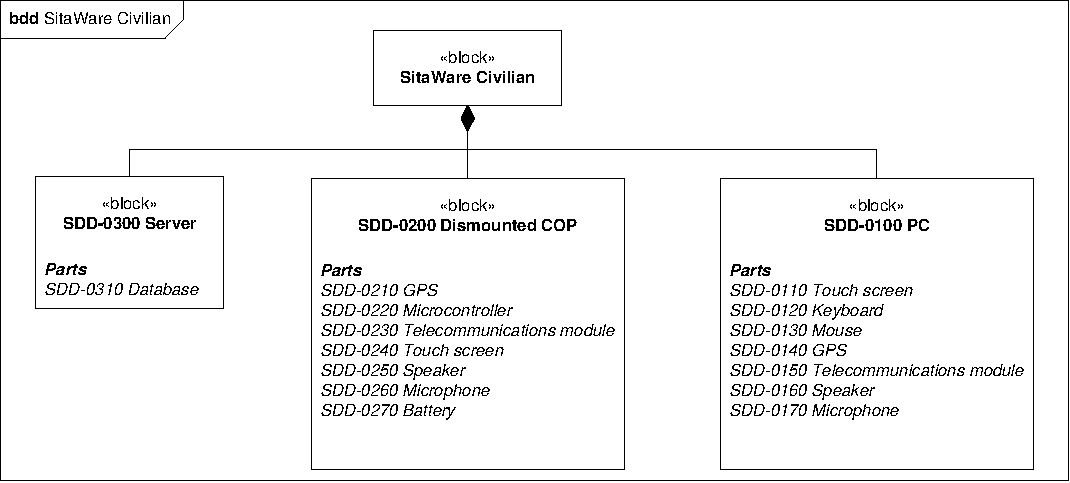
\includegraphics[width=0.95\textwidth]
{Billeder/background/bdd_overordnet.pdf}
\caption{Block Definition Diagram of the SitaWare Civilian system}
\label{fig:system_bdd}
\end{figure}

Figure \ref{fig:system_bdd} shows the block definition diagram for the SitaWare Civilian system. The block consists of three lower level blocks. A Server with a database, a hand-held device called Dismounted COP, and a PC. The Dismounted COP and PC both have several hardware and communication modules which are essential for the working system.

\begin{figure}[H]
\centering
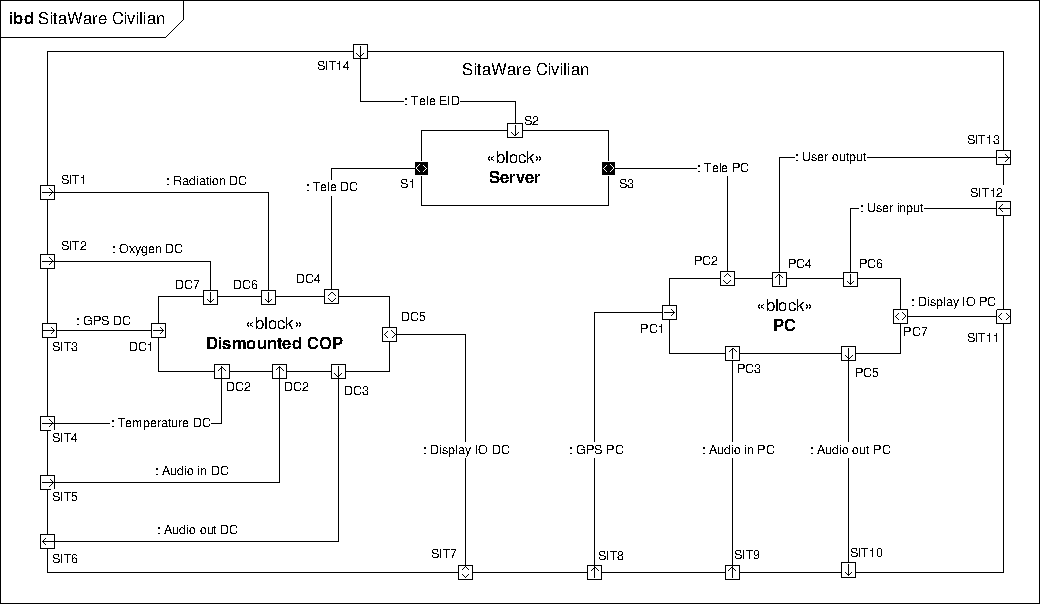
\includegraphics[width=0.95\textwidth]
{Billeder/background/ibd_overordnet.pdf}
\caption{Internal Block Diagram of the SitaWare Civilian system}
\label{fig:system_ibd}
\end{figure}

Figure \ref{fig:system_ibd} shows the internal block diagram for the SitaWare Civilian system. It shows the different internal and external interfaces for each part of the system. The data transfer descriptions provide some overview of how the communication in the system should be working, and which external systems and devices the system must interface to.

